\documentclass{article}
\usepackage[utf8]{inputenc}
\usepackage{graphicx}
\usepackage{amsmath}
\usepackage{amsfonts}
\usepackage{amssymb}

\usepackage{listings}
\usepackage{hyperref}

\newcommand{\mail}[1]{{\href{mailto:#1}{#1}}}


\begin{document}
\title{RandomFruitDB}
\author{Tristan Henchoz, Arthur Morgan, Mattéo Bonvin
	\\ {\small\mail{tristan.henchoz@unifr.ch, arthur.morgan@unifr.ch, matteo.bonvin@unifr.ch}}}
\date{\today}

\maketitle
\tableofcontents
\pagebreak


\section{Problem Statement}

RandomFruitDB is a distributed database system using the Elixir programming language. A distributed database is a database that is distributed across multiple computers, usually connected through a network. In a distributed database system, data is stored and managed in multiple physical locations, each with its own database management system (DBMS). The goal of a distributed database is to provide users with the ability to access and modify data from anywhere while providing fault tolerance and data availability.

Distributed databases differ from traditional centralized databases because they are designed to handle large amounts of data. Data and high-level consensus support distribution processes and distribution decision-making processes. They also typically provide features such as data partitioning and replication that allow data to be stored and accessed in multiple locations to improve performance and reliability.

This type of database faces a number of challenges. Firstly, they are more complex to set up, maintain, and troubleshoot than traditional single-server databases. In addition, they can potentially suffer from performance problems due to their complexity. Another major challenge they face is data consistency. They must ensure that data updates from one computer are correctly applied to all other computers. Finally, scalability is an issue for a distributed database because adding new computers adds complexity and can result in performance losses.

With RandomFruitDB, we try to solve these problems with the Chord algorithm. Peer-to-peer file sharing systems use the Distributed Hash Table (DHT), which is a Chord algorithm. Even though the network is constantly being joined and left, this allows the network to efficiently access and receive information from other networks. Each node has a unique ID. A large number is usually chosen from a random distribution. Each ID is higher than the previous one and lower than the next in a logical hierarchy. This space is called the code space. A list of other nodes in the network is maintained in a table called a fingerprint. A hash table is used to route data requests in the network.

When a person wants to join the network, they send a request to another person to find a successor. The location of the new node is reflected in its fingerprints. To receive data from the network, a node checks the data store to see if it is available. The request is sent to the next highest queue ID. If the data is not in the network, this process is repeated. The ability to efficiently manage nodes entering and leaving the network is an important feature of the Chord Algorithm. The proxy takes and updates the finger table when a node is offline. The finger table is updated when a new node joins the network. The Chord is an efficient way to access and get information from each other. It is used in many distribution systems.
\cite{reference_1}

\begin{figure}[h]
\centering
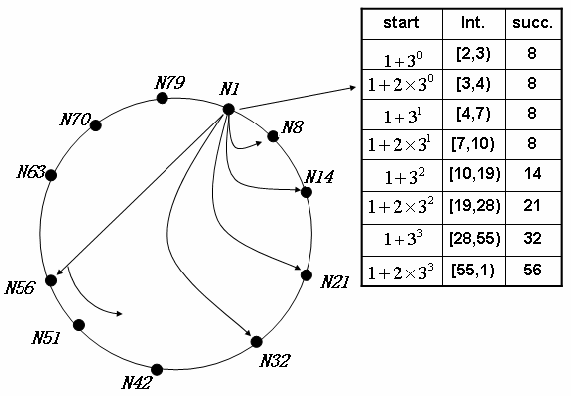
\includegraphics[width=\textwidth]{img/ChordAlgorithm}
\caption{A Bidirectional Chord System Based on Base-k Finger Table}
\label{figure 1}
\end{figure}

\pagebreak

\section{State-of-the-art}

Distributed databases are designed to store and manage large amounts of data across multiple servers, typically in a cluster or a grid. They allow for high availability, scalability, and fault tolerance by distributing the data and processing workload across multiple nodes.
There are several different types of distributed databases, including:
\begin{enumerate}
\item NoSQL distributed databases: These databases are designed to handle large amounts of data that may be structured, semi-structured, or unstructured. They often use non-relational data models, such as key-value stores, document stores, and column-family stores.
\cite{reference_2}

Examples include MongoDB, Cassandra, and HBase.
\item Relational distributed databases: These are traditional database management systems (DBMS) that have been extended to support distributed storage and processing. Examples include MySQL Cluster and Oracle RAC.
\item NewSQL distributed databases: These are a newer class of databases that combine the scalability and high performance of NoSQL databases with the Atomicity, Consistency, Isolation and Durability (ACID) properties and SQL interface of traditional relational databases . Examples include CockroachDB and TiDB.
\cite{reference_3}

\end{enumerate}
Another way to classify distributed databases is by the way they store and replicate data:
\begin{enumerate}
\item Shared-nothing architecture: In this type of distributed database, each node operates independently and has its own local storage. Data is partitioned and distributed among the nodes, and there is no central coordination or shared resources. This allows for high scalability and fault tolerance but can make it more difficult to maintain consistency and integrity. Examples include Cassandra and HBase.
\item Shared-nothing architecture with distributed consensus: In this type of distributed database, multiple nodes operate independently and have their own local storage, but they use a distributed consensus protocol to ensure data integrity and consistency. This allows for high scalability and fault tolerance, as well as strong consistency guarantees. Examples include Google Cloud Spanner and CockroachDB.
\item Shared-disk architecture: In this type of distributed database, multiple nodes share access to a common storage system, such as a SAN (storage area network). Data is partitioned and distributed among the nodes, but each node can access the data stored on the shared disk. This allows for easier maintenance of consistency and integrity but can be less scalable and less tolerant to failures. Examples include Oracle RAC and Sybase IQ.
\end{enumerate}
Our system would therefore be part of the NoSQL distributed databases with a Shared-nothing architecture

\pagebreak

\section{Presentation of the solution}

Our solution bypass a number of rule to create a real chord system for simplification. A big simplification is the order of the node and the file classification, as it is done randomly to avoid dealing with hash calculation. The solution is therefore simple, but it keeps its academic purpose.

A big simplification on our side is the creation and the use of a "dispatcher", which manage to add a new node in the ring and manage data communication with the ring. This system is purely here for simplification, and doesn't have any academic interest.

Our simplified node will connect directly to the dispatcher when created, and the later will assigned to them a position in the ring. The node will then take care to notify the other node of its presence. Our ring could in part refresh and correct its state (next node) on its own, but the feature wasn't turn on to avoid unexpected error as it is not fully fonctionnal.

The main part of our system is the possibility to retreive data. To store a file is simple, as the dispatcher select a node randomly to store it (to avoid the use of a hash table). To retreive some data, the dispatcher will randomly ask a node. The node will either answer with the file, otherwise it will ask its next node. A condition is put to avoid circular search, and when a file is found it is send directly to the dispatcher and does not circle back.

\section{Validation \& evaluation of the solution}

Our solution is currently not working, mainly because of the treatment of files using Elixir. But we manage to create a ring, being to store data (currently file names only) on multi node, and to retreive this data without having to connect to the node on which the information is located. 


\section{Discussion of the results}

As our solution doesn't create a finished and out-of-the box system, it reachs its mains points and can be further developp.


\pagebreak

\begin{thebibliography}{9}
\bibitem{reference_1}
Minghui Ji, "Hierarchical Bidirectional Chord," 2010 International Conference on Educational and Information Technology, 2010, pp. V3-486-V3-489, doi: 10.1109/ICEIT.2010.5607543.
\bibitem{reference_2}
Y. Zhou, Q. Chen, B. Shan, F. Jiang and Y. Pang, "A Distributed Storage Strategy For Trajectory Data Based On Nosql Database," IGARSS 2019 - 2019 IEEE International Geoscience and Remote Sensing Symposium, 2019, pp. 3487-3490, doi: 10.1109/IGARSS.2019.8900482.
\bibitem{reference_3}
K. Kaur and M. Sachdeva, "Performance evaluation of NewSQL databases," 2017 International Conference on Inventive Systems and Control (ICISC), 2017, pp. 1-5, doi: 10.1109/ICISC.2017.8068585.
\bibitem{reference_4}
Image Reference : H. Yan, Y. Jiang and X. Zhou, "A Bidirectional Chord System Based on Base-k Finger Table," 2008 International Symposium on Computer Science and Computational Technology, 2008, pp. 384-388, doi: 10.1109/ISCSCT.2008.55.
\end{thebibliography}

\pagebreak

\appendix

\section{Readme}

\lstinputlisting{src/backend/README.md}

\end{document}
